\section{Introduction}
\label{s:intro}


\wajih{I see some inconsistent Notations in this section. Please make sure that in this section all notations are up to date.}


\wajih{Is there a difference between Semantic Harmonization or \wordvec Harmonization? You use \wordvec harmonization here and Semantic Harmonization in Design section. Let's use consistent terminology throughout the paper. }

\wajih{There is a word "categorized ensemble learning" in the evaluation paragraph that is never described before in the intro. Let's use consistent wording througout the intro and throughout the paper. Also, in the Design section if you need to change the headings/titles to match with the intro, please do that. It is really hard to match the Intro section with the Design section.}

%\wajih{I have updated the macro logs as it does not make sense to use \ logs for just "system". I have changed the macro to "system logs". Make sure the paper is consistent with that.}

% The effectiveness of IDSes hinges on their ability to accurately detect these threats, maintain low false positive rates, and operate with minimal resource consumption, ensuring system performance is not compromised.

%\wajih{Give the workflow of MSSP and cite that organizations outsource their security. If you find any numbers on how many comapnies use MSSP and outsource their security operations that would be great. If you find any realworld attack examples on MSSP where the data was leaked that would be great as well. }



Intrusion Detection Systems (\ids) are crucial for countering Advanced Persistent Threats (APTs) in enterprises, as evidenced by major attacks, such as Solar Winds~\cite{solarwinds} and NotPetya~\cite{notpetya}. Given their stealth and persistence, many enterprises rely on Managed Security Service Providers (MSSPs) to improve their defenses. A survey~\cite{msspsurvey} involving over 5,000 IT professionals reported that about 75\% of companies use MSSPs. These providers integrate their security systems with clients' systems to manage \logs, typically configuring the clients' systems to transmit \logs to the cloud for analysis. Figure~\ref{mssp} illustrates this MSSP operational architecture.



Recently, Provenance-based IDS (\pids)~\cite{streamspot,provdetector2020,wang2022threatrace,shadewatcher,yangprographer,han2020unicorn,jia2023magic,flash2024,cheng2023kairos,sigl} have emerged as a highly effective means of enhancing intrusion detection. These systems leverage the extensive contextual information provided by \logs to bolster their detection capabilities. \pids operates by converting \logs into provenance graphs, which are then analyzed using machine learning techniques, such as Graph Neural Networks (\gnnshort), to identify and learn patterns of benign activity. By continuously monitoring these patterns, \pids can detect deviations that may indicate potential security threats. Upon detecting such anomalous graph patterns, the \pids generates alerts to prompt further investigation.

\smallskip
\PP{Limitations of Existing \pids}
\smallskip

\noindent
Despite \pids potential, the current operational mode of MSSPs and the state-of-the-art \pids face significant challenges in the complex landscape of enterprise security, which are described below.


\noindent
\textit{1. Privacy Risks \& Centralized Dependency.} Current \pids rely on a centralized infrastructure, requiring client machines to transmit their logs to a central server. This centralization is essential for aggregating large datasets to enable advanced deep learning techniques that effectively model and understand benign behaviors. However, it introduces significant privacy risks, as logs often contain sensitive information such as URLs visited, IP addresses, and application usage, which can be exposed in centralized systems. These privacy risks are not hypothetical; they have been emphasized in a recent Datadog report~\cite{datadog}. Further, training models on data from a single machine proves inadequate. As demonstrated by our experiments with \flash~\cite{flash2024} on the DARPA \optc dataset~\cite{darpaoptc}, performance dropped by 40\% in F-score when using single-host data compared to multi-host data.

    
\smallskip
\noindent
\textit{2. Scalability and Operational Inefficiencies.}  Centralized \pids face critical challenges with network overhead and scalability. Transmitting large volumes of logs for intrusion detection imposes high costs on users and organizations. Modern systems can produce gigabytes of logs daily~\cite{inam2023sok,hossain+depend}. Our analysis of \flash~\cite{flash2024} and \kairos~\cite{cheng2023kairos} using the \optc dataset, detailed in Section~\ref{cost_metric}, highlights these issues. Organizations similar in scale to those in the \optc dataset generate up to 1000 GB of logs daily, leading to significant network expenses. Users with limited bandwidth face difficulties uploading such large amounts efficiently. As the number of hosts grows, centralized \pids experience log congestion, causing bottlenecks that slow intrusion detection. Centralization incurs significant storage overhead, demanding constant resource allocation for growing data. Evaluations of \flash and \kairos reveal severe log congestion using \optc dataset, with \flash taking 27.7 hours and \kairos 56.6 hours to process a single day's logs, highlighting scalability limitations.


\begin{figure}[t!]
  \centering
  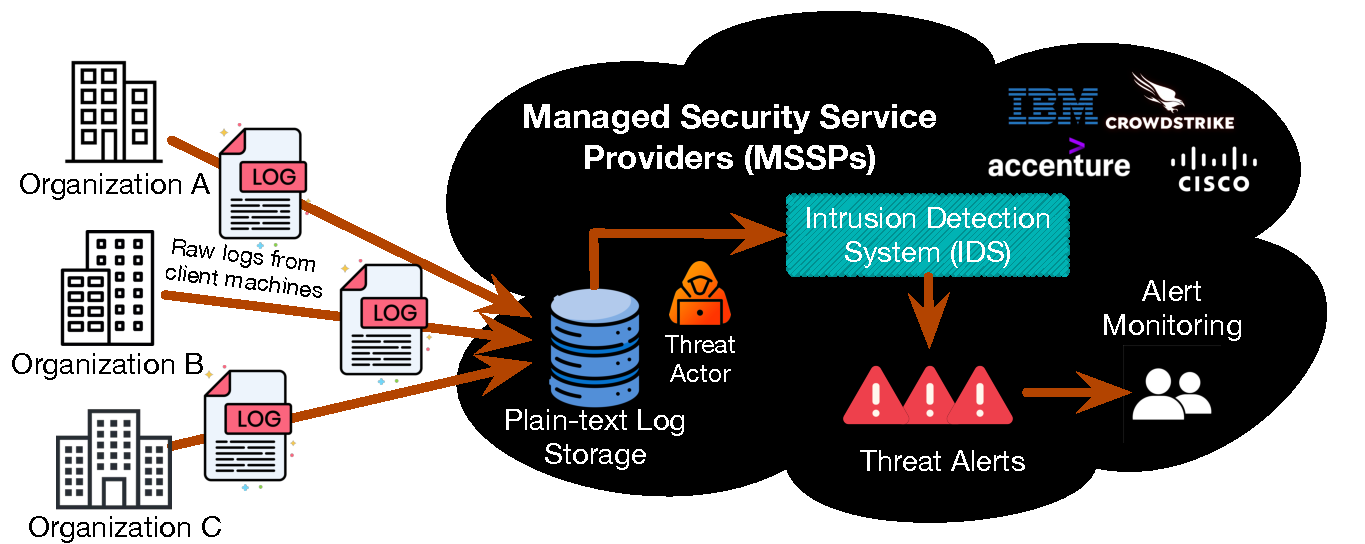
\includegraphics[width=0.32\textwidth]{fig/mssp.pdf}
  \caption{The MSSP architecture for intrusion detection collects plain-text system logs in a centralized storage managed by the MSSP. These system logs are then analyzed for intrusions. The architecture risks privacy leaks if a threat actor or a curious analyst within the MSSP accesses the data. \wajih{let's add cloud around MSSP and remove the big rectangle.}}
  \label{mssp}
  \vspace{-4ex}
\end{figure}

\smallskip
\PP{Our Approach \& Contributions}
\smallskip

%\wajih{Add one or two sentences at the relevant place to justify why we used graph-based anomlay detection with FL. Or in other words why FL alone is not sufficient}
\noindent
We introduce \Sys, a novel privacy-preserving \pids that integrates provenance graph representation learning with Federated Learning (FL) to address the challenges in applying FL to \pids. Prior work~\cite{wang2022threatrace} has shown the effectiveness of graph representation learning on provenance graphs for threat detection, as opposed to applying machine learning techniques~\cite{chowdhary2020natural, goodfellow2020generative} directly on system logs~\cite{deeplog2017, xia2019loggan}. Building on this insight, \Sys leverages Federated Provenance Graph Learning, combining FL’s decentralized architecture with powerful graph representation learning to capture the intricate relationships among system entities. {\bf To the best of our knowledge, \Sys is the first system to build a privacy-preserving \pids and effectively solve these challenges.} In \Sys, client logs remain local, ensuring that sensitive data never leaves the client's environment. Each client independently trains \gnnshort models, which are aggregated on a central server with models from other clients. This approach captures diverse activity patterns without transmitting actual logs, minimizing network overhead. Only model updates—mere kilobytes per client—are transmitted, greatly reducing the network burden. All major computations, including training, take place locally on client machines, leveraging their resources for real-time threat detection. This decentralized approach allows \Sys to scale effectively as more hosts are added, with each utilizing its own computing power and storage.

However, applying FL to \pids introduces several significant challenges, as summarized below:

\begin{enumerate}[itemsep=0.1em, parsep=0em, topsep=0em, leftmargin=*]
  \labitem{C1}{itm:c1}{\it Data Imbalance \& Heterogeneity Among Clients.} Variations in data distribution and volume across clients, often non-IID~\cite{zhao2018federated}, pose challenges in training a global model \( GNN_{Global} \) that performs uniformly well. Heterogeneous data resulting from different client applications can lead to suboptimal performance~\cite{qu2022rethinking}, and data imbalances can cause models to be biased towards clients with more extensive datasets, potentially overlooking unique patterns in less-represented clients~\cite{duan2020self}. This issue is critical for \pids, as a biased \( GNN_{Global} \) may result in high false alarms, undermining detection accuracy.

  \labitem{C2}{itm:c2}{\it Feature Space Heterogeneity.} Inconsistent encoding of identical features across clients leads to difficulties in model convergence and reduces the effectiveness of federated averaging. \pids, such as \flash~\cite{cheng2023kairos}, utilize a \wordvec model to encode semantic attributes within a provenance graph. Due to the inherent randomness of the \wordvec algorithm, identical tokens \( t \) are encoded into different vectors \( v_i(t) \) by each client \( i \), using their local feature sets \( \mathcal{F}_i \). This variability disrupts the convergence and efficacy of local \gnn models \( \text{GNN}_{i} \) and complicates federated averaging for the global \gnn model \( \text{GNN}_{\text{Global}} \), leading to suboptimal anomaly detection performance, as detailed in \cite{zhou2023fedfa}.

  \labitem{C3}{itm:c3} {\it Temporal Misalignment.} Aggregating temporal graph models from clients with temporally misaligned data challenges the creation of a cohesive global model. Systems like \kairos \cite{cheng2023kairos} employ temporal graph neural networks (TGN) to trace the evolution of system provenance graphs. However, federated learning's application across fragmented and misaligned client data impedes effective federated averaging, leading to improper alignment when aggregating models trained on diverse temporal datasets. This results in a loss of temporal information and hinders the formation of a cohesive global model \( GNN_{Global} \).
  
  % \labitem{C4}{itm:c4} {\bf Non-Privacy-Preserving Data Structure.} Existing \pids frameworks often use data structures that do not preserve privacy, making them unsuitable for integration with FL.
\end{enumerate}

% \wajih{The next three paragraphs are the most important part of your paper. Make sure you highlight all the different features of your system including Process Entity Categorization, Semantic featurization, GNN based anomaly detection. And if there are other features of your paper mention them here as well.}

\wajih{This paragraph one of the important paragraphs. make sure you highlight all the features of your systems in this paragraph.}

\wajih{Use consistent terminology with the Design section.}

To address ~\ref{itm:c1}, we have designed a novel ensemble learning framework \Fix{(Section~\ref{})}. In this framework, each submodel is trained to specialize in learning system activities associated with specific process entities, which are standardized across all clients. This standardization is facilitated by a sophisticated categorization scheme enabled by our dual-server architecture. Through this system, process entities from all clients are organized into \textit{K} privacy-preserving bins. Each client then aligns its process nodes with these bins, constructs a provenance subgraph for each bin, and trains a \gnnshort model on these graphs. The models from all clients are then aggregated into \textit{K} model pairs, forming a comprehensive global ensemble model set. This strategic approach ensures that models with similar data distributions are merged effectively, thereby maintaining the integrity of unique activity patterns across diverse client environments. We compared our methods with existing solutions such as FedProx~\cite{li2020federated} and FedOpt~\cite{asad2020fedopt} for addressing heterogeneity in FL settings and found that our techniques outperform these existing solutions, as detailed in Section~\ref{sec:fedalternatives}.

\wajih{In the following paragraph, make sure that you use consistent terminology that you used in the design section like harmonization, featurization, categorization. This paragraph one of the important paragraphs. make sure you highlight all the features of your systems in this paragraph.}


To tackle ~\ref{itm:c2}, we implement a \wordvec harmonization scheme utilizing a dual-server architecture \Fix{(Section~\ref{})}. In this setup, a central server issues encryption keys to clients, allowing them to securely encode \wordvec tokens. Subsequently, a utility server processes these encrypted tokens to achieve a unified, privacy-preserving vector representation. This method ensures that sensitive data remains protected while facilitating accurate and consistent semantic encoding across different clients. To avoid the problem of \ref{itm:c3} arising from the use of temporal graph networks, \Sys employs an inductive graph neural network model~\cite{hamilton2017inductive}, which has been shown by prior work~\cite{flash2024,shadewatcher,wang2022threatrace} to offer good performance and is less affected by temporal dependencies \Fix{(Section~\ref{})}. This approach mitigates the issues of temporal misalignment that arise in federated learning for intrusion detection settings.

%\wajih{make sure that the numbers are correct below.}
We evaluated \Sys using open-source datasets from \darpa, including E3~\cite{error3}, E5~\cite{bug5}, and \optc~\cite{anjum2021analyzing}, which cover a wide range of attack scenarios and system behaviors. Since existing state-of-the-art \pids already achieve near-perfect detection accuracy, {\bf the primary goal of \Sys is to demonstrate that a privacy-preserving \pids can be built while maintaining similar performance.} Our results show that \Sys achieves detection performance with an average precision of 96\% and recall of 97\%, matching the accuracy of state-of-the-art \pids. What distinguishes \Sys is its ability to deliver this accuracy while significantly reducing privacy risks and improving scalability in enterprise settings. Experiments were conducted to investigate the effectiveness of \wordvec harmonization and \Fix{categorized ensemble learning} in addressing the data heterogeneity issue. These methods were found to significantly enhance detection performance compared to the vanilla approach.

%\wajih{Do we have any new results after last submission. If yes, add sentences related to those results as well.}

\Sys achieves a 170-fold reduction in network communication costs compared to existing centralized systems. Moreover, the decentralized nature of \Sys allows for much faster inference times, bounded only by the client with the most data, completing the full \optc dataset in a few minutes, whereas existing \pids, such as \flash and \kairos, require several hours. We present a comprehensive analysis of our system's resilience against various adversarial attacks in Section~\ref{sec:adversarial}. Additionally, we provide a detailed analysis of the privacy protection offered by our system in Section~\ref{sec:privacy}. We also compare our technique to existing solutions for dealing with heterogeneity in the FL setting in Section~\ref{sec:fedalternatives}. Furthermore, we provide an extensive ablation study, comparison of our approach to alternate privacy techniques, such as differential privacy and benchmark of various encryption methods for use in our system in Appendix~\ref{app:ablation}.

% The main contributions of our work are as follows:

% \begin{itemize}[topsep=.1ex,itemsep=-.1ex,leftmargin=*]
%     \item[--] To the best of our knowledge, we are the first to introduce federated provenance graph learning in the domain of IDS with our system, \Sys.
%     \item[--] We have introduced a novel \textbf{ensemble learning} and \textbf{process entity categorization} framework for dealing with diverse heterogeneous client data distributions.
%     \item[--] We developed a sophisticated \textbf{\wordvec harmonization framework} using a multi-server architecture for secure private aggregation of semantic attributes.
%     \item[--] We conduct a comprehensive evaluation of our technique on real-world datasets, demonstrating \Sys's effectiveness in detecting system threats while being scalable and privacy-preserving.
% \end{itemize}

%\url{https://anonymous.4open.science/r/TrustWatch}

% \begin{table}[t!]
%   \centering
%   \scriptsize
%     %\caption{Limitations of existing \pids. \wajih{Add in caption that which \pids are not specified in the table and why.}}
%     \caption{Existing \pids limitations. \flash and \kairos outperform other existing \pids systems ~\cite{wang2022threatrace,han2020unicorn,streamspot,yangprographer,shadewatcher,provdetector2020}. Also, they all suffer from data privacy leakage issues. Therefore, we have excluded these \pids from the table. }
%     \setlength{\tabcolsep}{10pt}
%       \begin{tabular}{ | c | c | c | c |}

%         \hline
%              & \bf Data & \bf Network  & \bf Scalability \\
%              & \bf  Privacy & \bf  Overhead &  \\
%         \hline
%         \hline
%         \disdet~\cite{dong2023distdet} & NO                       & LOW      & HIGH       \\
%         \hline
%         \flash~\cite{flash2024}     & NO            & HIGH             & MEDIUM      \\
%         \hline
%         \kairos~\cite{cheng2023kairos}     & NO            & HIGH             & LOW         \\
%         \hline
%         {\bf\Sys}  & YES                & LOW               & HIGH        \\
%         \hline
%       \end{tabular}
%       \label{tab:limitations}
%   \end{table}
